%!TEX output_directory = <<temp>>
%!TEX copy_output_on_build = true

\documentclass[11pt]{article}

\usepackage[utf8]{inputenc}

\usepackage{amsmath}		% lets you input equations in math mode
\usepackage{graphicx}		% lets you include images
\usepackage{enumerate}		% lets you make lists
\usepackage{hyperref}		% lets you make links
\usepackage{subcaption}     % if you want to use subcaptions
\usepackage[all]{hypcap}	% makes links refer to figures and not captions
\usepackage{relsize}		% lets you use relative font sizes
\usepackage{caption}        % lets you add captions
\usepackage{array}          % lets you specify table column widths
\usepackage{cite}
\usepackage{float}
\usepackage{array}
\usepackage{cellspace}
\usepackage[margin=1in, paperwidth=8.5in, paperheight=11in]{geometry} %

% oooOhmmmmmmmmmm
\newcommand{\megaOhm}{M$\Omega$}
\newcommand{\kiloOhm}{k$\Omega$}
\newcommand{\ohm}{$\Omega$}
\newcommand{\microFarad}{$\mu$F}

\setlength\cellspacetoplimit{8pt}
\setlength\cellspacebottomlimit{8pt}
\newcommand\cincludegraphics[2][]{\raisebox{-.3\height}{\includegraphics[#1]{#2}}}

% place graphics in ./img/
\graphicspath{ {img/} }

\begin{document}



\title{Title}
\author{Bogdan Vitoc}
% \date{date here} % leave this commented to display the current date
\maketitle



\begin{abstract}
    Maecenas sed diam eget risus varius blandit sit amet non magna. Praesent commodo cursus magna, vel scelerisque nisl consectetur et. Lorem ipsum dolor sit amet, consectetur adipiscing elit.
\end{abstract}


\section{Sit Ultricies Malesuada Nibh}

Integer posuere erat a ante venenatis dapibus posuere velit aliquet. Donec ullamcorper nulla non metus auctor fringilla.

% Example figure 1
\begin{figure} [H] % H: forces layout according to position in the source
	\centering

	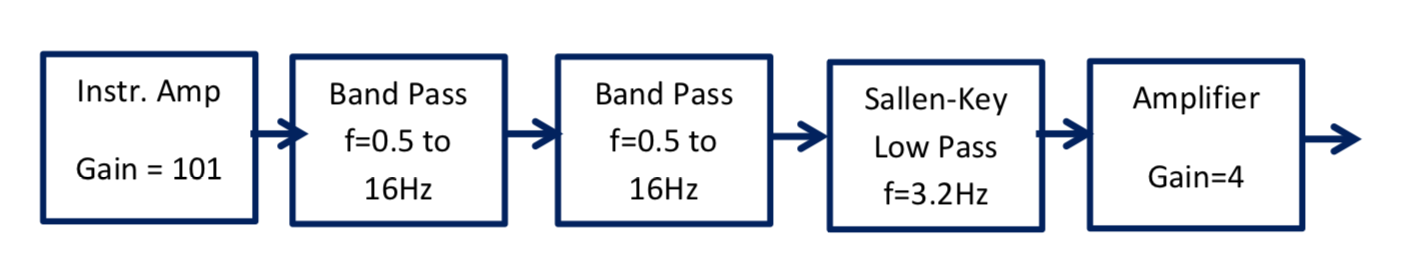
\includegraphics[width=0.8\textwidth]{block_diagram}

	\captionsetup{margin={0.2\textwidth,0.2\textwidth}}
	\caption{Sed posuere consectetur est at lobortis.}
	\caption*{\small (Egestas Justo Commodo)}
\end{figure}


\section{Etiam Sollicitudin Vehicula}

Duis mollis, est non commodo luctus, nisi erat porttitor ligula, eget lacinia odio sem nec elit.

% Example figure 2
\begin{figure} [H]
	\centering

	\includegraphics[width=0.8\textwidth]{circuit}

	\captionsetup{margin={0.2\textwidth,0.2\textwidth}}
	\caption{Duis mollis, est non commodo luctus, nisi erat porttitor ligula, eget lacinia odio sem nec elit.}
\end{figure}


\end{document}